\documentclass[12pt,a4paper]{article}
\usepackage{spex450_documents}

\title{An introduction to data analysis and MATLAB}

\author{Peter Lamb}

\date{Week 1}

\begin{document}

\maketitle

\section{Data analysis}
Data analysis, an unavoidable part of all experimentation and research, is often the postgrad student's greatest consumer of time and a major source of frustration.  
Consideration of analysis methods and the available tools is often left to the last minute when important decisions (or mistakes!) have already been made.

The aim of this section of the paper is to introduce and build skills and confidence in a number of useful data analysis tools.  
Such skills are highly sought after in a wide variety of postgraduate and employment opportunities.

\subsection{Raw data}
Raw data are the original, unfiltered, unprocessed data that you record during the data collection.  
These data (note: \emph{data} is plural and \emph{datum} or \emph{data point} is the singular form) are important and you should treat them so.  
Keep these original data files in a safe location and do not touch them.  
Make copies of these originals and then perform any analysis on the copies.  
This way, if you make any mistakes during your analysis you can always go back, make new copies of the originals and begin again.
Raw data files should never be edited, this is not only poor practice but also unethical.

\subsection{Naming convention}
Two students, A and B, both test four participants twice, once before an intervention session and once after.  
The data file names from the two are shown below:

\begin{table}[H]
  \begin{center}
    \begin{tabular}{|l|l|}
    \hline
    \multicolumn{2}{|c|}{Student A} \\
    \hline
    Jonesy1.dat & Jonesy2.dat \\
    \hline
    Mike-T1.dat & Mike2.dat \\
    \hline
    Richard\_1.dat & Rich2.dat \\
    \hline
    Bill\_1.dat & Bill\_2.dat \\
    \hline
    \end{tabular}
  \end{center}  
  \label{tab:namingconventionsa}
\end{table}

\begin{table}[H]
  \begin{center}
    \begin{tabular}{|l|l|}
    \hline
    \multicolumn{2}{|c|}{Student B} \\
    \hline
    JM\_T1.dat & JM\_T2.dat \\
    \hline
    MF\_T1.dat & MF\_T2.dat \\
    \hline
    RB\_T1.dat & RB\_T2.dat \\
    \hline
    WN\_T1.dat & WN\_T2.dat \\
    \hline    
    \end{tabular}
  \end{center}
  \label{tab:namingconventionsb}
\end{table}

To describe the naming convention for Student B you would say: use two letters, one for the first letter of the first name and one for the first of the surname, an underscore `\verb|_|' and then the test number i.e. T1 for test 1 and T2 for test 2.  
Now look back and try to describe the convention for Student A.

Why is this important?  
File names are often a useful way of recording important information about what went on in the data collection session.  
You may include information like; participant name/id, experiment type/condition, trial number etc.  
For example, the name `PP1\_G3\_T7.dat' could be used to indicate Participant 1, Group 3 and Trial 7.  
During the exercise in this module you will learn how to create automated data analysis processes to remove repetitive steps.  
You will learn how to write instructions for a computer to follow to process the data for you (you may be familiar with this already when using macros in Excel).  
In the case of Student B, you could instruct the computer to look at the first two characters to get the name of the subject and the fifth, or last, character to get the test number.  
You would have a difficult job instructing anyone how to extract information from the data file names used by Student A's convention!

\subsection{Take note}
When you are collecting data it is useful and often critical to record all available information about the testing session.  
Record information such as sample rate, amplifier and filter settings, data channel names, equipment serial numbers, tester names, session date and time etc.  
All this information can be used to track down or exclude any errors/anomalies that may occur during data collection.

\subsection{Analysis software}
After the data have been collected there will almost always be a number of processes that need to be completed before the results of the investigation can be presented.  
There could be multiple participants, trials, conditions and variables that may need to be cleaned, filtered and averaged before any statistical analysis can be used to determine an outcome.  
The data may also need to be collated from a number of separate locations and various different file formats.

These processes will undoubtedly be far too onerous to be done manually and you will need to find a software package to assist you.  
A familiar and easy to use program such as Microsoft Excel is often the first choice for most analysis procedures.  
This can be sufficient if the requirements are basic and the amount of data is minimal.  
However, it can be hugely time consuming and computationally inadequate for larger data sets and more complex analysis procedures.

There are other software programs available that are written specifically to facilitate powerful, repeatable and rapid data analysis.  
Unfortunately, as always, all of the benefits are not without some disadvantages.  
These software programs often require a period of learning before they can become useful.  
However, the goal of this module is to show that it is worth it!

\section{MATLAB -- \emph{The Language of Technical Computing}}
\label{sec:matrices}
The name MATLAB (note: always written in all caps) stands for Matrix Laboratory and as the name suggests almost all the work done in MATLAB is based upon the manipulation of matrices.  
Therefore, it is important to get a basic understanding of what a matrix is, why they are so useful and how MATLAB uses them to tackle some applicable data analysis.

\subsection{Scalars, vectors, matrices, arrays and structures}
In MATLAB a basic \textbf{matrix} is a rectangular array of numbers, arranged in rows and columns (rows $\times$ columns).  
The simplest matrix, a single number in a $1\times1$ (1 row by 1 column) arrangement, is known as a \textbf{scalar}.  
A single row or column of values is known as a \textbf{vector}.

%% interactive additions here:

A scalar ($1 \times 1$):
\[3\]

A row vector ($1 \times 5$):
\[ \left[ \begin{array}{ccccc}
3 & 12 & 5.1 & 9 & 7.02 \end{array} \right]\]\\

A column vector ($5 \times 1$):
\[ \left[ \begin{array}{c}
3 \\
12 \\
5.1 \\
9 \\
7.02 \end{array} \right]\]\\

A matrix ($4 \times 3$):
\[ \left[ \begin{array}{ccc}
3 & 12 & 5.1\\
12 & 1 & 11.04\\
5.1 & 13 & 3.8\\
9 & 7.5 & 8 \end{array} \right]\]\\

You will be familiar with displaying data in rows and columns when using a spreadsheet, such as Microsoft Excel.  
Rows and columns are a very effective way of displaying data in readiness for further analysis.  
Table {\ref{tab:laptimes} shows the lap split times and maximum and minimum speeds for a 10-lap running race.  

\begin{table}[H]
  \begin{center}
    \begin{tabular}{cccc}
    \toprule
    Lap & Lap Time (s) & Maximum speed (ms$^{-1}$) & Minimum speed (ms$^{-1}$) \\
    \midrule
    1 & 67.4 & 7.2 & 2.4 \\
    2 & 68.2 & 6.3 & 5.5 \\
    3 & 70.1 & 6.1 & 5.3 \\
    4 & 70.4 & 5.9 & 5.1 \\
    5 & 69.3 & 6.3 & 5.7 \\
    6 & 71.2 & 5.8 & 5.0 \\
    7 & 73.8 & 5.7 & 4.9 \\
    8 & 75.2 & 5.5 & 4.5 \\
    9 & 73.4 & 5.6 & 5.2 \\
    10 & 71.1 & 8.7 & 4.8 \\
    \bottomrule    
    \end{tabular}
  \end{center}
  \caption{Lap times and speeds for a 10-lap running race \label{tab:laptimes}}  
\end{table}

The data could be stored in a matrix as shown in Figure \ref{fig:lapmatrix}.

\begin{figure}[H]
	\[ \left[ \begin{array}{cccc}
	1 & 67.4 & 7.2 & 2.4 \\
    2 & 68.2 & 6.3 & 5.5 \\
    3 & 70.1 & 6.1 & 5.3 \\
    4 & 70.4 & 5.9 & 5.1 \\
    5 & 69.3 & 6.3 & 5.7 \\
    6 & 71.2 & 5.8 & 5.0 \\
    7 & 73.8 & 5.7 & 4.9 \\
    8 & 75.2 & 5.5 & 4.5 \\
    9 & 73.4 & 5.6 & 5.2 \\
    10 & 71.1 & 8.7 & 4.8 \end{array} \right]\]	
	\caption{The data from the Table \protect \ref{tab:laptimes} stored in a 10x4 matrix \label{fig:lapmatrix}}	
\end{figure}

This matrix, with rows and columns, is a two-dimensional (2D) matrix.  
It is possible to have multi-dimensional matrices and when we have more than three dimensions it can become very hard to visualise these arrangements.  
For a 3D matrix, in a $3\times3\times3$ arrangement, the elements could be visualised as a simple rubix cube as shown in Figure \ref{fig:3dmatrix}.  
The three dimensions could be described as rows, columns and \emph{blocks} of these rows and columns.  
The highlighted element would be in row 2, column 3 of block 2 (taken from the nearest top left corner).

\begin{figure}[H]
\begin{center}
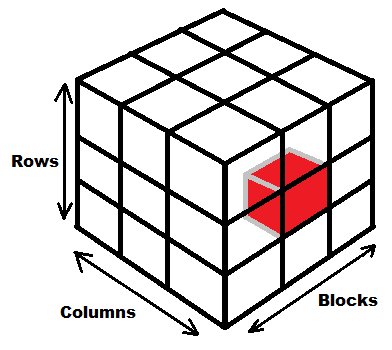
\includegraphics[width=0.8\textwidth]{3x3cube.png}
\caption{Visualising a 3-dimensional matrix}
\label{fig:3dmatrix}
\end{center}
\end{figure}

Figure \ref{fig:5dmatrix} shows a possible visualisation of a 5D matrix.  
We could imagine a collection of cubes, arranged themselves in rows and columns - a $2\times3\times3\times3\times3$ matrix.  
To describe the highlighted element we could say; within the cube in row 2, column 2, take the element in row 1, column 3 of block 1.

It is possible to have a multi-dimensional dataset that is made up from simple parameters you may use in a standard research project.  
For example: 10 participants are in a study with 7 conditions;  
8 trials are completed for each condition in 6 separate testing sessions;  
during each trial, 11 signals are recorded consisting of 4,000 data points each.  
This could produce a 6D matrix in a $10\times7\times8\times6\times11\times4000$ arrangement but it is not worth imagining how this might look!!

\begin{figure}[H]
\begin{center}
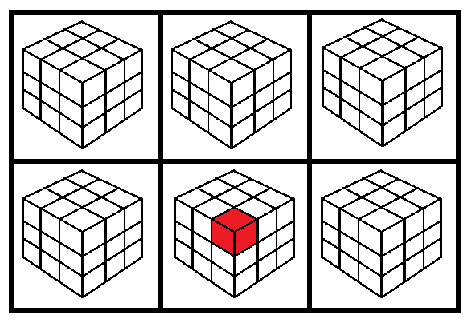
\includegraphics[scale=0.5]{2x3cubes.png}
\caption{Visualising a 5-dimensional matrix}
\label{fig:5dmatrix}
\end{center}
\end{figure}

In MATLAB, an \textbf{array} is a collection of variables (these could be text, scalars, vectors, matrices, etc.) as opposed to a matrix which is a collection of numbers.  
For example, an array could be used to store a number of matrices.  
Figure \ref{fig:matrixarray} shows an array containing three items.

\begin{figure}[H]
	\[ \left\lbrace 
		\begin{array}{ccc}
		\left[ \begin{array}{cccc}
			12 & 5 & 7 & 3 \\
			2 & 3 & 20 & 9 \\
			15 & 6 & 8 & 11 \\
			4 & 1 & 21 & 18 \end{array} \right] &
		\left[ \begin{array}{cccc}
			2 & 13 & 9 & 7 \\
			12 & 11 & 20 & 16 \\
			4 & 9 & 8 & 8 \\
			17 & 6 & 19 & 1 \end{array} \right] &
		\left[ \begin{array}{cccc}
			2 & 12 & 4 & 1 \\
			17 & 14 & 2 & 21 \\
			6 & 19 & 10 & 9 \\
			22 & 5 & 16 & 18 \end{array} \right]
 		\end{array}
 	\right\rbrace \]
	\caption{An array containing three $4 \times 4$ matrices}
	\label{fig:matrixarray}
\end{figure}

A \textbf{structure} is probably the most complicated item you will come to use in MATLAB.  
A structure is a collection of related data, often in different forms (scalars, text, matrices etc).  
For example, a subject of an experiment could be seen as a structure, `SUBJECT'.  
Associated with this subject is their name (text), their age, height and weight ($1\times3$ matrix) and their test data of 10 samples of 5 variables ($10\times5$ matrix).  
This structure is shown in Figure \ref{fig:structure} as an example.  

\begin{figure}[H]
    \begin{center}
        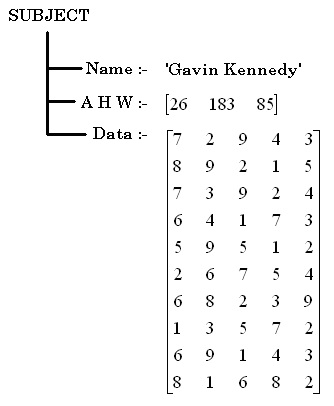
\includegraphics[width=0.8\textwidth]{subject.png}
        \caption{An example of a structure}
        \label{fig:structure}
    \end{center}
\end{figure}

A \textbf{structure} variable can also be arranged to store a collection, or array, of individual structures.   
Figure \ref{fig:structurearray} shows the array of structures, called SUBJECT, containing two items.

\begin{figure}[H]
\begin{center}
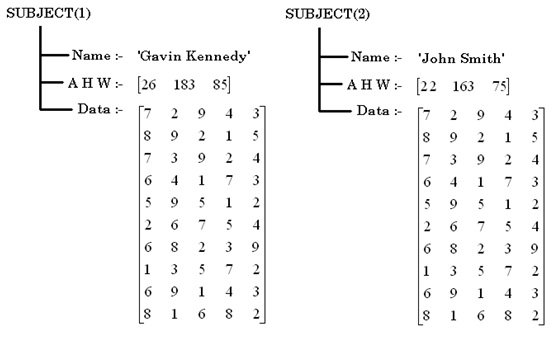
\includegraphics[width=\textwidth]{subject_array.png}
\caption{Two structures that make up the structure array called SUBJECT}
\label{fig:structurearray}
\end{center}
\end{figure}

\subsection{An introduction to MATLAB}
MATLAB has a vast collection of functions and resources, making finding the one that may be useful to you seem very daunting.  
However, there are a number of different ways of getting to grips with what is available.

The product help is a good way of browsing through the catalogue of resources.  
Open the \textbf{Product Help} by clicking the \textbf{Help} dropdown list from the HOME ribbon and selecting \textbf{Support Web Site}\footnote{The exact layout and naming of buttons and menu items may vary slightly depending on the operating system and version of MATLAB you are running.}.  
From here you can search by typing relevant key words in the search box or simply browse through the functions in the documentation.  
There is also a \textbf{Learn MATLAB} button that takes you to a list of self-paced courses that may be helpful getting you accustomed to working with MATLAB – the \textbf{MATLAB Onramp} would provide a good introduction.

Another, less formal, option is to search popular internet forums. 
General searches, such as ``how to index vector elements in matlab'', will likely result in you being directed to the online MATLAB documentation; however, more specific queries will likely bring you to Forums such as \href{https://stackoverflow.com/}{stackoverflow}, \href{https://stackexchange.com/}{stackexchange} or MATLAB's own forum – \href{https://au.mathworks.com/matlabcentral/}{matlabcentral}.
matlabcentral also hosts many user-contributed functions on their File Exchange that can be downloaded and run for your own purposes.

%In addition to the built-in MATLAB functions you will begin to create your own custom functions and scripts.  
%It is a good idea to create a directory somewhere on your computer specifically for your custom functions.

%In order to use these functions as if they were standard functions we need to instruct MATLAB where to find them.  
%We must add this directory path to the list of paths that MATLAB will search through.
%The following steps may vary depending on the computer, MATLAB version and permissions:
%\begin{itemize}
%	\item Within the \textbf{Home} tab, click the \textbf{Set Path} button.
%	\item Click \textbf{Add Folder...} and choose the correct directory (or select \textbf{Add with Subfolders...} if you have functions in nested folders).
%	\item Click \textbf{OK} on the \textbf{Path Warning} dialog if it appears.
%	\item The directory should have been added to the top of the list of MATLAB search paths.  Click \textbf{Save}.
%	\item MATLAB may now ask if you want to save the \textbf{pathdef.m} file to another location.  Click \textbf{Yes} and then \textbf{Save} to save the file to the default location.
%	\item Click \textbf{Close} to return to MATLAB.
%\end{itemize}

Please watch the following MATLAB demonstration videos before continuing.  
These can be found by searching for ``Getting Started with MATLAB'' in the `Search Documentation' box in the top right corner.
You should see the following videos listed under \textbf{Videos}.

\begin{enumerate}
	\item Getting Started with MATLAB
	\item Working in the Development Environment
\end{enumerate}

\end{document}